We conduct our study in a large scale open source software system to distinguish Defect Debt and Bugs. First, we analyze the history of issues in the system, and then we suggest a definition to Defect Debt and to Bugs. Based on this definition we quantify  both on them per release. Second, we analyze the evolution of Defect Debt to understand its impact on future feature addition. Third, based on our metrics we propose a model to Defect Debt.

\vspace{3mm}
\noindent\rqi
\vspace{3mm}

\noindent\textbf{Motivation:} Technical Debt is a broad concept and can be classified in many subcategories (e.g., Design Debt, Documentation Debt, Defect Debt). However, these subcategories may not have a clear definition making difficult to distinguish them to already know terms (i.e, Defect Debt and Bugs). Answering this research question, will provide us a way to identify and quantify Defect Debt. 

\vspace{1mm}
\noindent\textbf{Approach:} To identify Defect Debt we first, mine the project issuer tracker to extract the bug reports. Then, we link the bug report to its respective software release using the reported date. 

Second, we extract the commits from the source code repository. In some projects like Google Chrome, it is a common practice to add the bug id in the commit message. Based on this knowledge, we use the commit messages to link the commits with bug reports. Regular expressions are the most common way to identify bug id in the commit message. This technique provide us the exact date that the bug was fixed, which is more precise than reeling on the closing date from the bug report. The trade-off of this technique is that is not always possible to find the bug id for each one of the bug reports, or the bug id in the message can be wrong as it is a manual input. Other than that, it is possible to find multiple commits that corresponds to the same bug id, scenario that need further investigation when linking. 

Third, we link the commit to its respective release using commit date. For each defect in our system we have the date that they were reported and the date they were fixed. 

Fourth, we take all reported defects for each one of the releases. Then, we group it based on the release they were fixed. In total we did this process for 26 Chrome releases. We plot the data to visualize the distribution of the defects and draw conclusions. 

\vspace{1mm}
\noindent\textbf{Result:} Analyzing the graphs shown in figure \ref{fig:defect_release_1} we observe that most defects are fixed during the release that they were reported or in the immediately next one. A smaller quantity of defects reported in the current release will remain in the system for a long time, but eventually get fixed. The observed pattern holds for each analyzed version. 

In some cases, like shown in figure \ref{fig:defect_release_6} we can observe a reopened bug. (i.e., the same defect has a fix reported in one previous release and in the current release as well). Just based in this argument, we can not say that we were able to identify all reopened bugs in the system. There are different factors that can impact this scenario (e.g., it is possible that a reopened bug has a new bug id in the issuer tracker, and in that case our approach would not identify it as a reopened bug). More investigation is needed in order to explain this phenomena in a satisfactory way. 

Accordingly with our findings, we say that it is possible to distinguish regular Bugs and Defect Debt based on their fix behavior. Bugs are more critical defects and are fixed near to its reported date (i.e., in the same or in the immediately next release), and Defect Debts are defects that lingers in the system for several releases but eventually are fixed. We believe that the fix behavior of the 

There is not hard proof in our study that the reason that Bugs are fixed first than Defect Debt because they are more critical, but based on our experience we argue that tasks in a project are assigned to developers following a priority order. Even considering a open source environment where non-core developers (e.g., an anonymous contributor), could be fixing bugs just because they are easy to fix, previous work \todo{cite appache work from peter} has shown that most of the development activity is done by the core developers of the system.

Based on our findings we quantify the average of Bugs and Defect Debt in the analyzed releases. Considering the reported defects on Chrome has an average of 69.55\% Bugs and 30.44\% of Defect Debt.

\conclusionbox{Bugs are more critical defects, and get fixed in the reported or in the next release. Whereas Defect Debt may linger in the system for a long time, but eventually it get fixed. The average percentage of Bugs is of 69.55\%, and Defect Debt is of 30.44\%}

 
\begin{figure}[thb!]
    \caption{Fix for defects reported in release 1.}
    \label{fig:defect_release_1}
    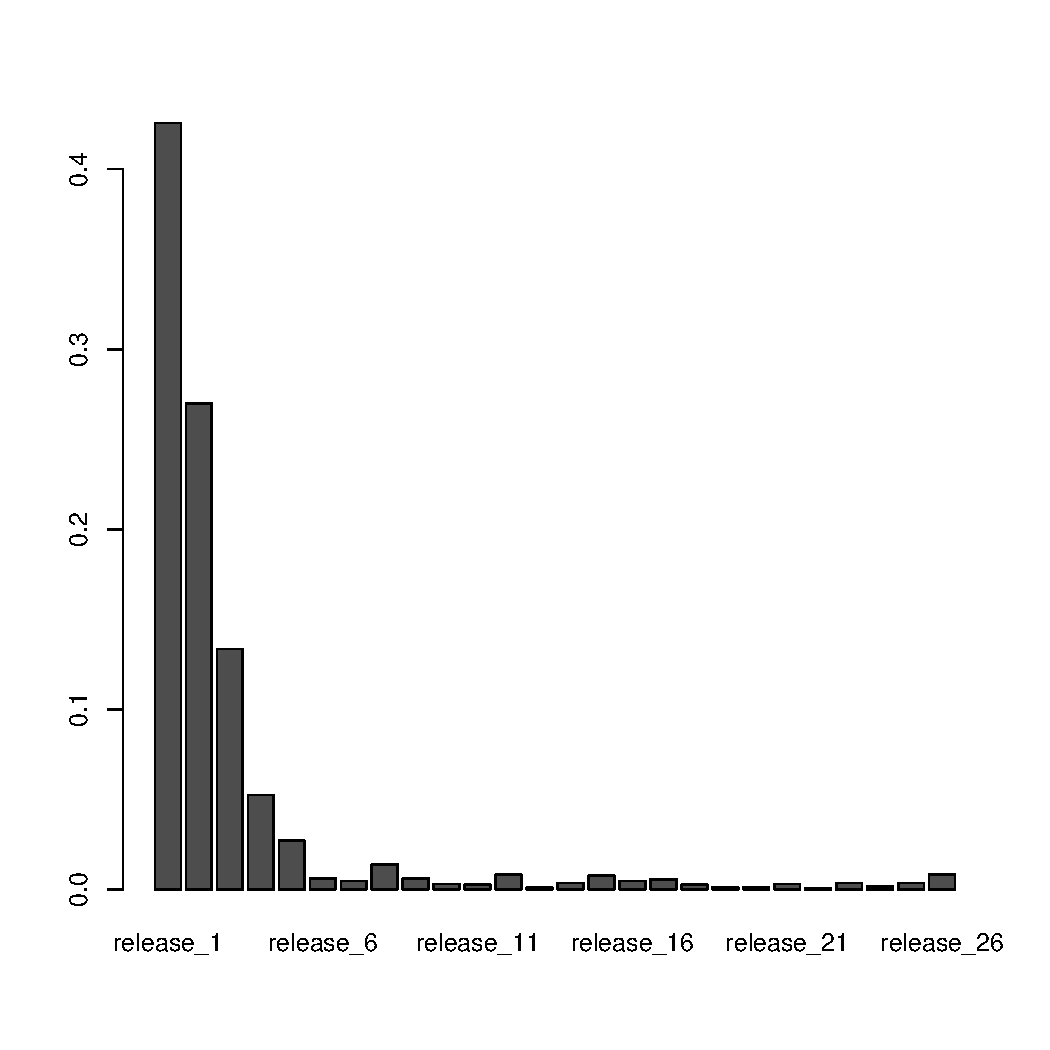
\includegraphics[width=90mm,scale=0.5]{figures/r1}
\end{figure}

\begin{figure}[thb!]
    \caption{Fix for defects reported in release 6.}
    \label{fig:defect_release_6}
    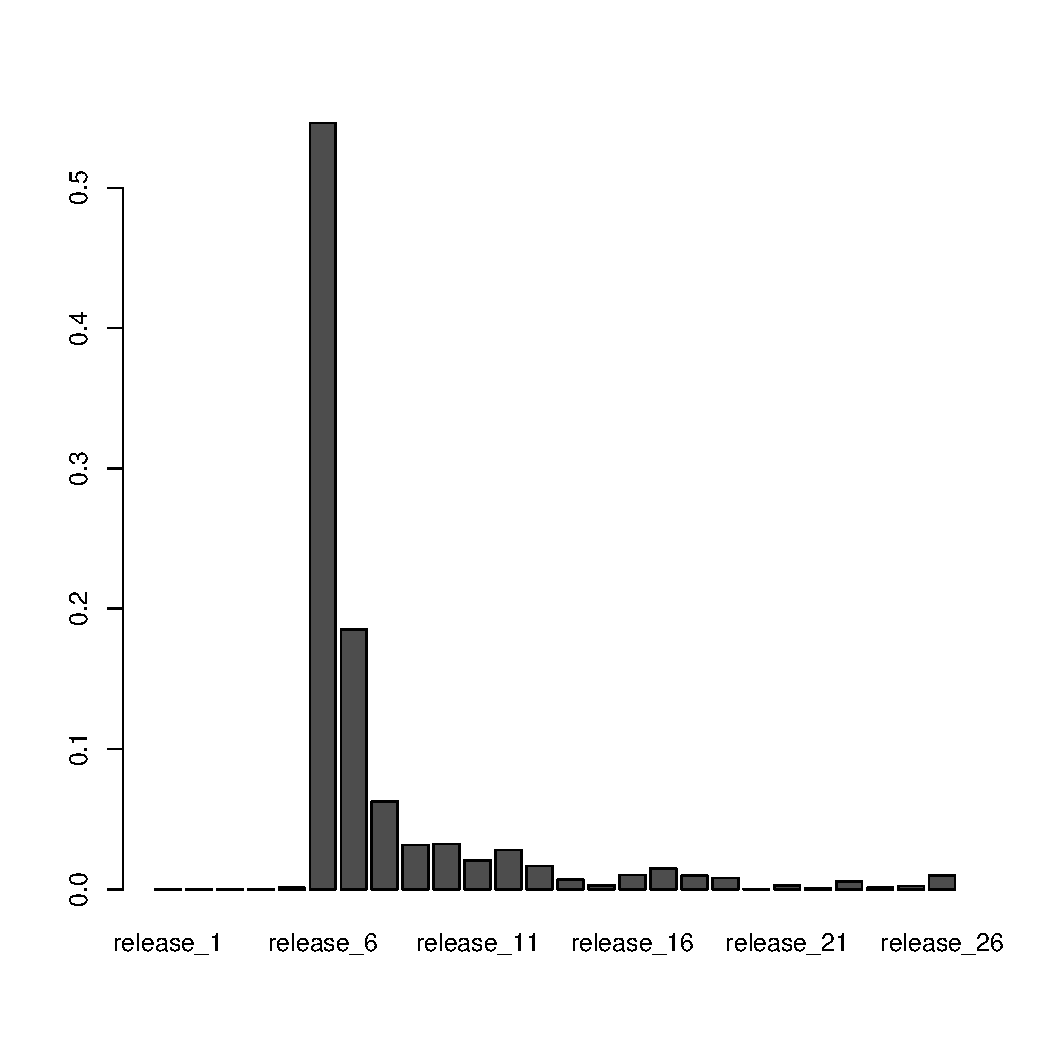
\includegraphics[width=90mm,scale=0.5]{figures/r6}
\end{figure}

\vspace{3mm}
\noindent\rqii
\vspace{3mm}

\noindent\textbf{Motivation:} Technical debt can bring you short term advantage in trade off maintenance costs in the  long run. which means that when well managed technical debt can be used as a tool to achieve projects goals. That been said, we want to know how much is too much when dealing with technical debt. We argue that the amount of technical debt starts to slow down your development is the point to pay off. 

\vspace{1mm}
\noindent\textbf{Approach:} Now that we have an approach to identify defect debt we want to see how it relates with the amount of changes in the project. First we quantify the number of defect debt in the software, then we mine the source code repository to examine the changes. We will find all the changes(commits) related to a specific release using the commit date. Analyzing the commit messages we will categorize the changes of the release to see with the change is due to a bug fix or adding new features. After this analyze we will have the number of commits that were bug fix and the number of commits that were new features. To measure if  a high number of defect debt is preventing new features to be implemented in the project, we analyze if the number of new features are reducing at the same time that the number bug fixes are increasing. We also should expect that a higher number of defects is reported when the number of technical debt is higher in the project.

\vspace{1mm}
\noindent\textbf{Result:} The number of open defects increases during the project life-cycle. Defect Debt has growth peaks, but eventually get removed in future releases. Analyzing the feature addition and the defect debt graph we found that the introduction of defect debt does not impact the number of  feature addition per release. 

\begin{figure}[thb!]
    \caption{Release density evolution}
    \label{fig:release_density}
    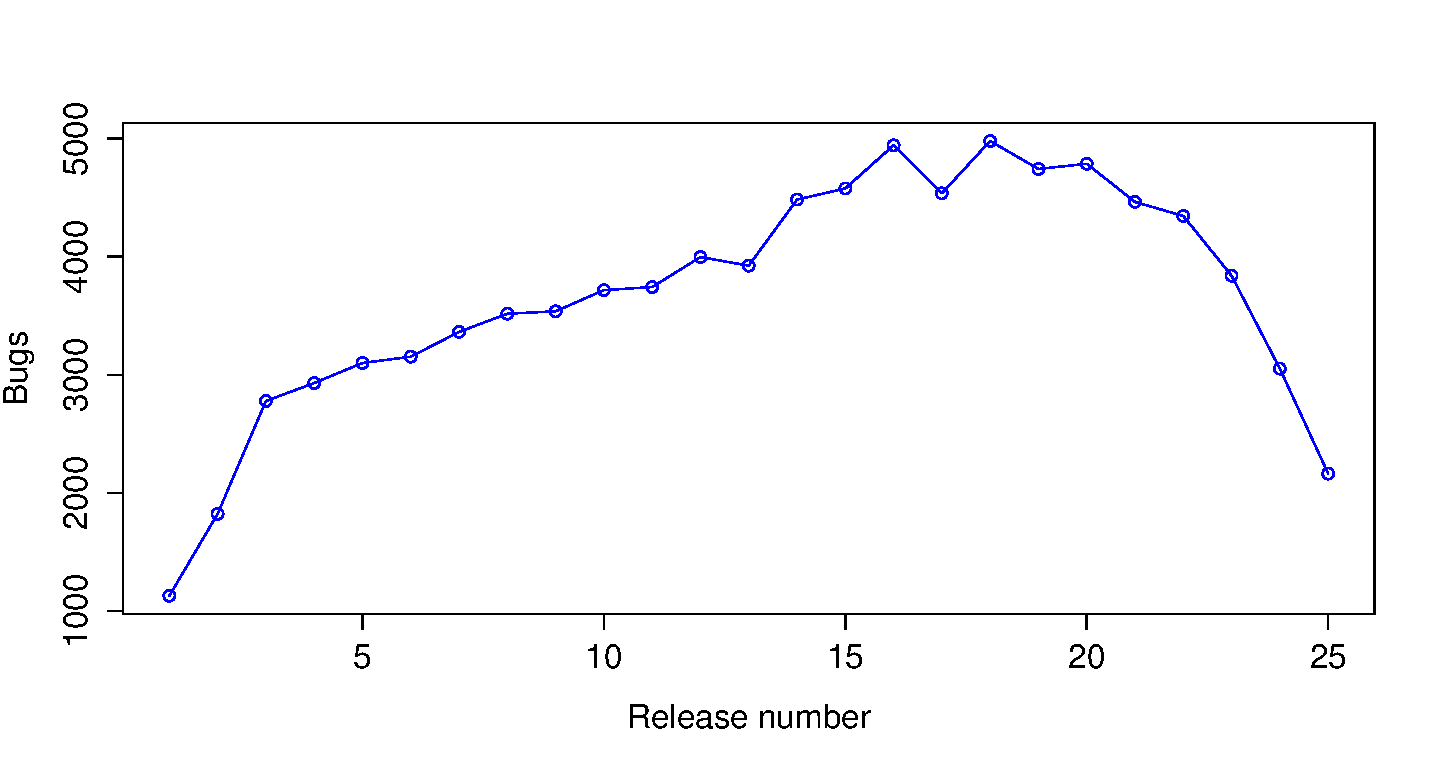
\includegraphics[width=90mm,scale=0.5]{figures/number_of_bugs_releases}
\end{figure}

\begin{figure}[thb!]
    \caption{Release density evolution}
    \label{fig:release_density}
    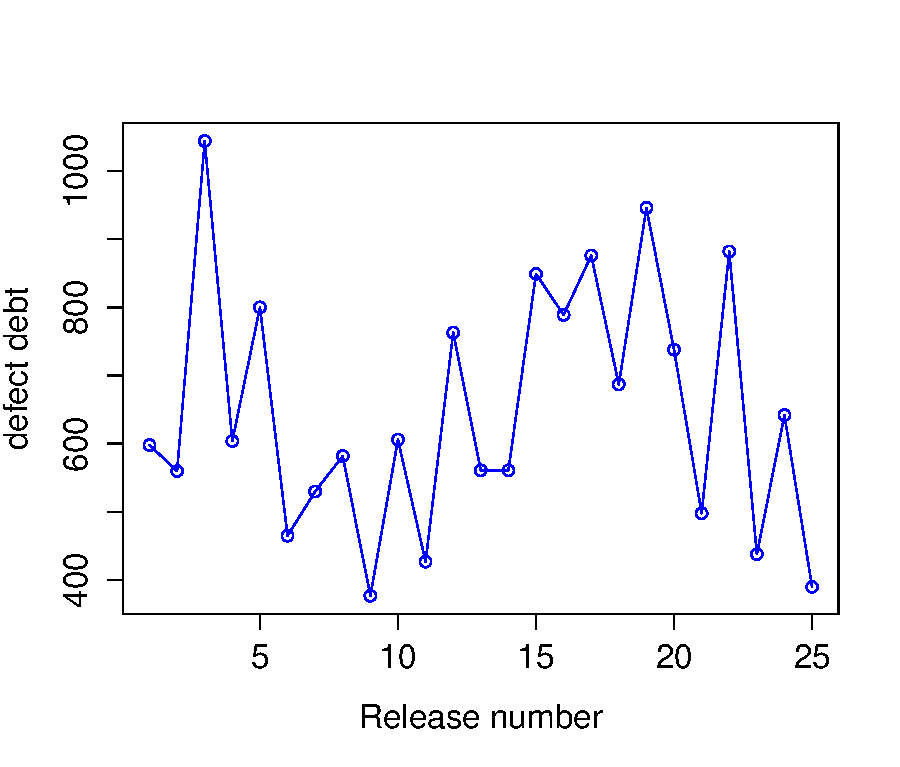
\includegraphics[width=90mm,scale=0.5]{figures/technical_debt}
\end{figure}

\begin{figure}[thb!]
    \caption{Release density evolution}
    \label{fig:release_density}
    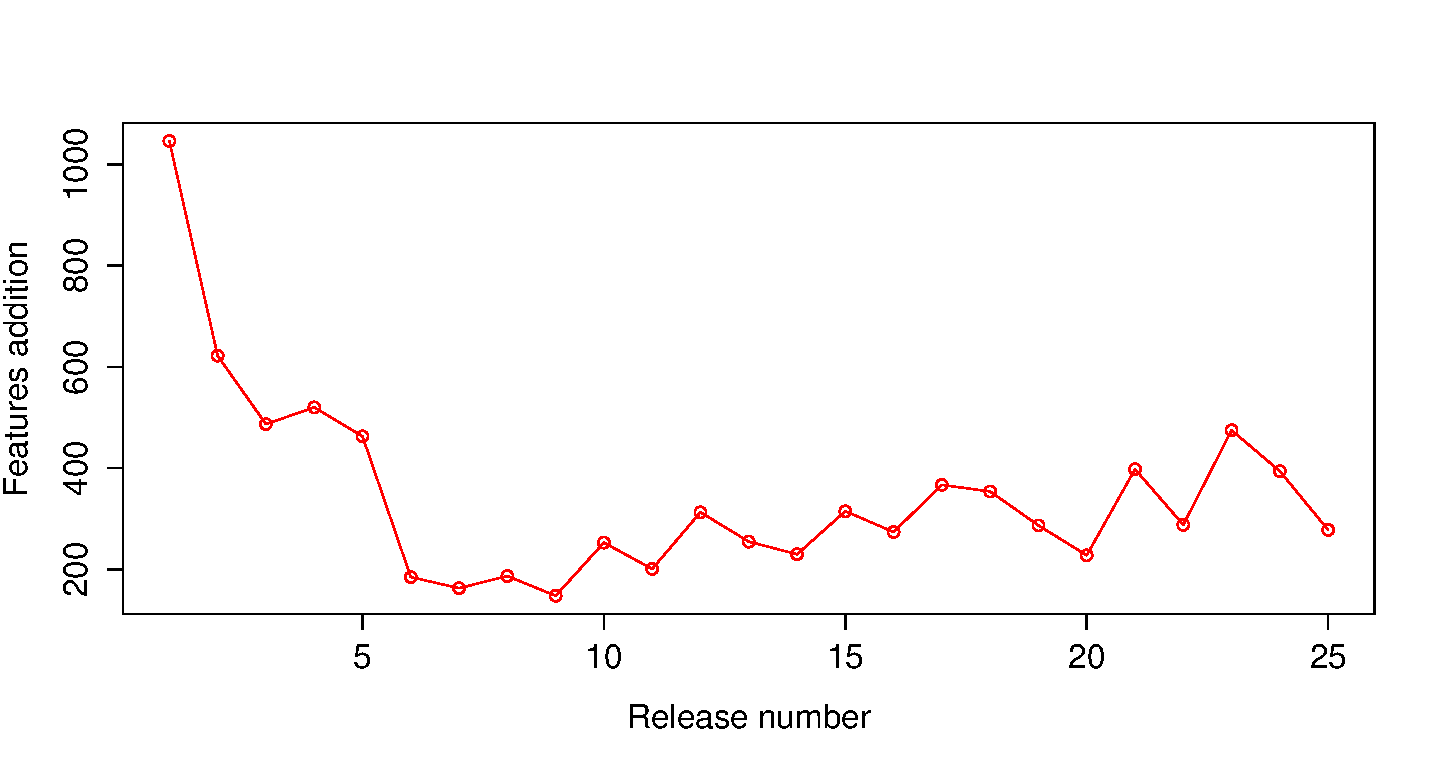
\includegraphics[width=90mm,scale=0.5]{figures/feature_addition_releases}
\end{figure}

\vspace{3mm}
\noindent\rqiii
\vspace{3mm}

\noindent\textbf{Motivation:} Learning from mistakes of the past can be useful in software engineering as well. We want to know if it is possible to determine if a defect are likely to become defect technical debt by analyzing the cases that were identified in RQ1. Answering this question will provide us with more means to effectively manage defect debt by knowing before hand that the specific defect will have to be handled in the future to avoid quality impacts. 

\vspace{1mm}
\noindent\textbf{Approach:} Based on the defect debt identified in the project we will analyze the bug reports looking for patterns in the attributes to build a prediction model. This information will serve as our training set. Then we will run the analyze again using the data from other project to measure the precision of our model. 

\vspace{1mm}
\noindent\textbf{Result:}